	
\begin{frame}
\frametitle{Fission}
  \begin{figure}[t]
   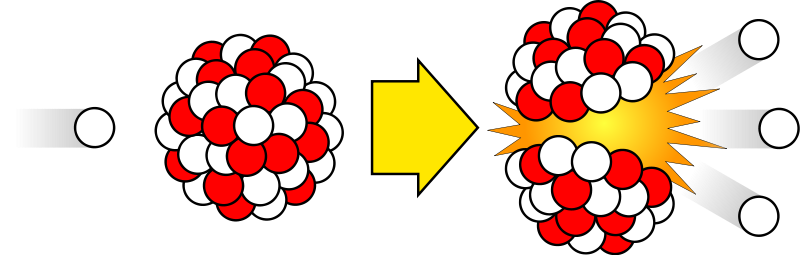
\includegraphics[width=\textwidth]{./images/fission.png}
	\caption{Cross sections: $\sigma(E,\vec{r},\hat{\Omega},T,x,i)$}
	\end{figure}
\end{frame}


\begin{frame}
\frametitle{Fission Chain Reaction}
  \begin{figure}[t]
   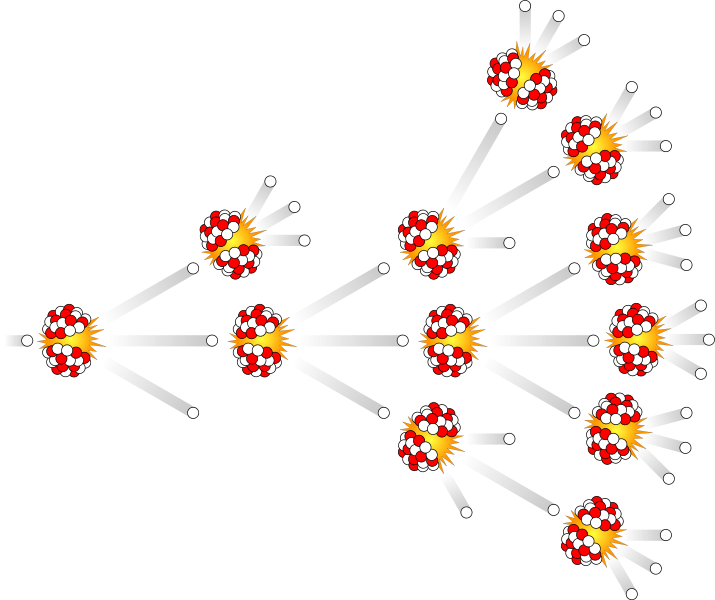
\includegraphics[height=0.75\textheight]{./images/fission-chain.png}
	\caption{Criticality: $k=1$}
	\end{figure}
\end{frame}

\begin{frame}
\frametitle{Reactivity}
		     \begin{align*}
		     k &= \mbox{"neutron multiplication factor"}\\
		     &= \frac{\mbox{neutrons causing fission}}{\mbox{neutrons produced by fission}}\\
		     \rho &= \frac{k-1}{k}\\
		     \rho &= \mbox{reactivity}\\
		     \end{align*}
\end{frame}

\begin{frame}
\frametitle{Feedback}
  \begin{figure}[t]
   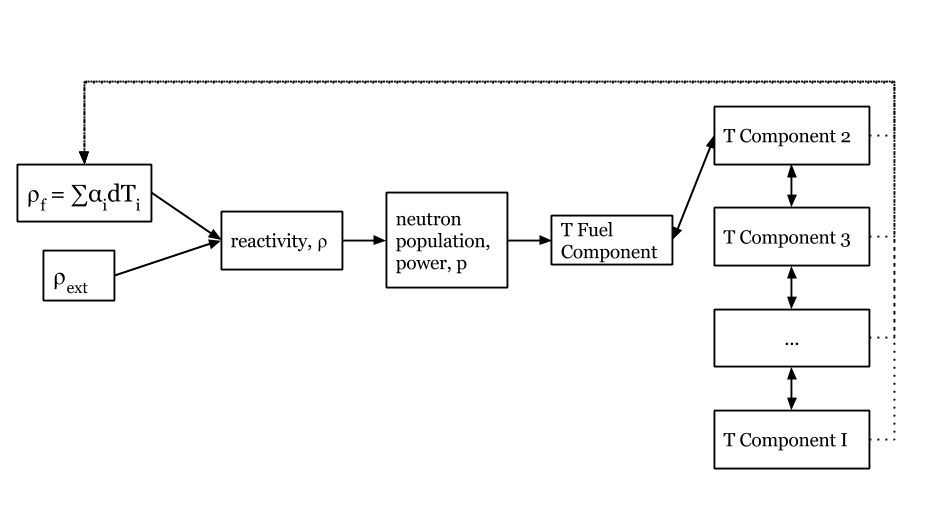
\includegraphics[width=0.75\textwidth]{./images/feedback.png}
	\end{figure}
\end{frame}


\begin{frame}
\frametitle{Kinetics with Delayed Neutrons}
  \begin{figure}[t]
   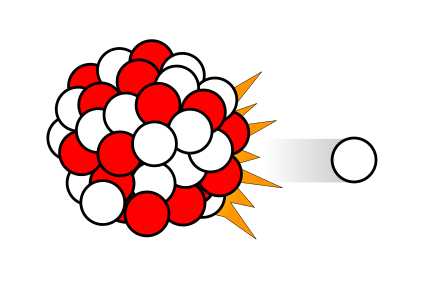
\includegraphics[height=0.75\textheight]{./images/delayed_neutron.png}
	\caption{Delayed neutron fraction, $\beta_i$, and corresponding decay constant, $\lambda_{d,i}$.}
	\end{figure}
\end{frame}

